\documentclass[12pt]{article}
\usepackage{hyperref} % 如果需要超链接功能
\usepackage{ctex} % 中文支持
\usepackage{tocloft}   % 用于控制目录格式(视情况看看是否需要这一行代码)
\usepackage{amsmath} % 数学公式支持
\usepackage{graphicx} % 图片支持
% https://liam.page/2014/09/08/latex-introduction/ 参考这个网站
\title{大四下学习笔记}
\author{杨昊}
\date{\today}
\begin{document}
% 生成标题
\maketitle
\thispagestyle{empty}  % 第一页不显示页码

\newpage
% 生成目录
\tableofcontents


\newpage

% 定义章节编号
\section{机器学习}


% 添加子目录(小节)
\subsection{理论}

\subsubsection{2025年2月25日:强化学习概念}
强化学习(Reinforcement Learning, RL)是一种机器学习方法,旨在通过与环境交互,使智能体(Agent)学习如何采取最优行动,以最大化某种累积奖励。它与监督学习和无监督学习不同,强调试错探索(Exploration-Exploitation)以及基于奖励信号的学习。
\begin{figure}[h]
    \centering
    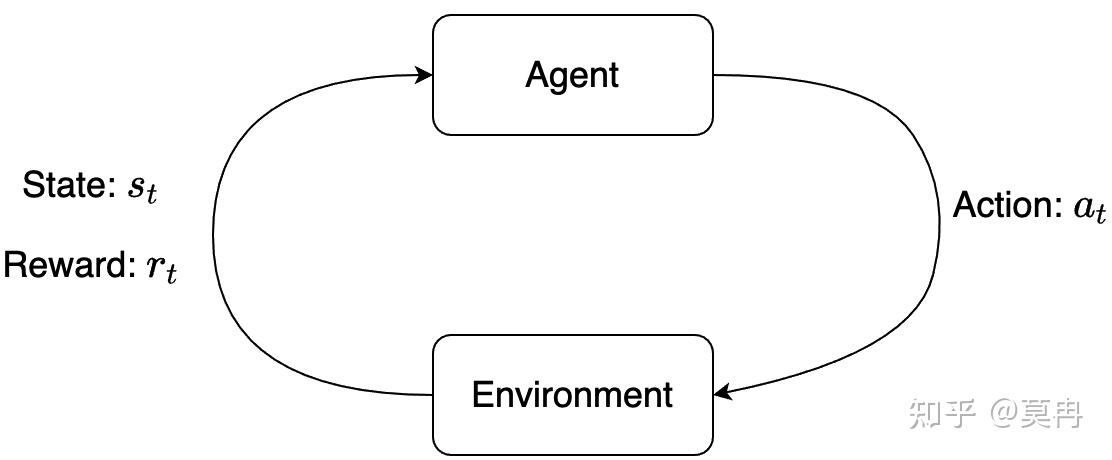
\includegraphics[width=0.7\textwidth]{./images/rlimage.jpeg}  % 图片文件名(包括路径)
\end{figure}

强化学习任务通常用马尔可夫决策过程来描述:机器处于环境$E$中,状态空间$X$,其中每个状态$x \in X$是机器感知到的环境的描述,机器能采取的动作构成了动作空间$A$,若某个动作$a \in A$作用在当前状态$x$上,则潜在的转移函数$P$将使得环境从当前状态按照某种概率转移到另一个状态,在转移到另一个状态的同时,环境会根据潜在的“奖赏”函数$R$反馈给机器一个奖赏。

机器要做的是通过在环境中不断地尝试而学得一个“策略”,根据这个“策略”在状态$x$下就能知道要执行得动作。

\textbf{在强化学习任务中,学习的目的就是要找到能使长期累积奖赏最大化的策略。}
\begin{quote}
强化学习与监督学习来说,强化学习是没有人直接告诉机器在什么状态下应该做什么动作,只有等到最终结果揭晓,才能通过“反思”之前的动作是否正确来进行学习,因此,强化学习在某种意义上可看作具有“延迟标记信息”的监督学习问题。
\end{quote}
\subsubsection{2025年3月1日:评估模型的指标及正则化与交叉验证}
\noindent\makebox[\linewidth]{\hrulefill\quad 评估模型的指标 \quad\hrulefill}

对于分类模型,我们通常使用精度、召回率、F1 分数等指标来评估模型性能。

在分类任务中,混淆矩阵的每个元素表示真实值与模型预测值之间的关系。对于二分类问题,混淆矩阵通常是一个 2x2 的矩阵,包含以下四个元素:
\begin{quote}
    \begin{table}[h]
        \centering
        \begin{tabular}{|c|c|c|}  % 定义三列,所有列都居中对齐,使用竖线分隔

            \hline
            {真正例 TP} & 实际为正类的样本被模型预测为正类 \\
            \hline
            {假正例 FP} & 实际为反类的样本被模型预测为正类 \\
            \hline
            {真反例 TN} & 实际为反类的样本被模型预测为反类 \\
            \hline
            {假反例 FN} & 实际为正类的样本被模型预测为反类 \\
            \hline
        \end{tabular}
    \end{table}

\end{quote}
F1分数是精度和召回率的调和平均数。
\begin{itemize}
    \item 准确率(Accuracy):$A = \frac{TP+TN}{TP+TN+FP+FN}$
    \item 查准率、精度(Precision):$P = \frac{TP}{TP+FP}$
    \item 查全率、召回率(Recall):$R = \frac{TP}{TP+FN}$
    \item F1 分数:$F1 = \frac{2 \times P \times R}{P + R}$
\end{itemize}
ROC 曲线是一种用于评估分类模型性能的工具。它是通过不同的分类阈值(threshold)来绘制的,横轴是假正例率(False Positive Rate, FPR),纵轴是真正例率(True Positive Rate, TPR),即召回率(Recall)。
\begin{itemize}
    \item 假正例率(FPR):$FPR = \frac{FP}{FP+TN}$,表示实际为反类的样本被模型预测为正类的比例。
    \item 真正例率(TPR):$TPR = \frac{TP}{TP+FN}$,表示实际为正类的样本被模型预测为正类的比例。
\end{itemize}
AUC 是 ROC 曲线下的面积,表示模型在各种阈值下的表现。AUC 值的范围从 0 到 1,AUC 越接近 1,说明模型的性能越好。AUC 为 0.5 时,表示模型的分类效果相当于随机猜测,即没有任何分类能力;而 AUC 为 1 则表示模型的分类能力完美,能够完全区分正类和负类。

对于回归问题,常用的评估指标包括 均方误差(MSE) 和 决定系数(R²)。
\begin{itemize}
    \item 均方误差(MSE):$MSE = \frac{1}{n} \sum_{i=1}^{n} (y_i - \hat{y}_i)^2$
    \item 决定系数(R²):$R^2 = 1 - \frac{\sum_{i=1}^{n} (y_i - \hat{y}_i)^2}{\sum_{i=1}^{n} (y_i - \bar{y})^2}$,值越接近1,表示模型的拟合效果越好。
\end{itemize}

\noindent\makebox[\linewidth]{\hrulefill\quad 正则化与交叉验证 \quad\hrulefill}


正则化(Regularization) 是一种用于\textbf{防止模型过拟合的技术}。它是结构风险最小化策略的实现,是在经验风险上加一个正则化项或罚项。
\begin{quote}
    当模型复杂度过高(如参数过多或深度过深的神经网络)时,可能会很好地拟合训练数据,但在测试数据上表现较差,导致泛化能力下降。正则化通过限制模型的参数大小或稀疏化参数,减少对训练数据的过度拟合,使其在未见数据上的表现更稳定。
\end{quote}
正则化一般具有如下形式:
$$min_{f \in F} \frac{1}{N} \sum_{i=1}^{n} L(y_i, f(x_i)) + \lambda J(f)$$
其中,第一项是经验风险,第二项是正则化项,$\lambda > 0$为调整两者之间关系的系数。

常见的正则方式有
\begin{itemize}
    \item L1正则化(Lasso):$J(f) = ||f||_1 = \sum_{i=1}^{n} |w_i|$,即所有参数的绝对值之和。
        \begin{itemize}
            \item L1 正则化可以使得模型的参数稀疏化,即许多参数为 0,从而减少模型的复杂度。
            \item 适用于高位稀疏数据。
        \end{itemize}
    \item L2正则化(Ridge):$J(f) = ||f||_2^2 = \sum_{i=1}^{n} w_i^2$,即所有参数的平方和。
        \begin{itemize}
            \item L2 正则化不会使权重变为 0,而是让它们趋近于 0,使模型更平滑,减少对训练数据的敏感性,提高泛化能力。
            \item 适用于大部分回归问题。
        \end{itemize}
    \item Dropout:在训练过程中,随机将一部分神经元的输出置为 0,从而减少神经元之间的依赖关系,防止过拟合。
    \item 早停(Early Stopping): 在训练过程中,当验证集上的误差不再下降时,停止训练,防止模型过拟合。
\end{itemize}
在数据不充足时,为了选择好的模型,可以采用交叉验证(Cross Validation)的方法。
交叉验证的基本想法是重复地使用数据,把给定地数据进行切分,将切分地数据集组合为训练集与测试集,在此基础上反复地进行训练、测试以及模型选择。
\begin{itemize}
    \item 简单交叉验证:将数据集划分为训练集和测试集,只进行一次划分。
    \item K 折交叉验证:将数据集划分为 K 个大小相似的互斥子集,每次用 K-1 个子集的并集作为训练集,余下的子集作为测试集,共进行 K 次训练和测试。
    \item 留一交叉验证:K 折交叉验证的特例,K 等于数据集的大小。
\end{itemize}

\subsection{实践}
dff
\section{有限元分析}

\end{document}
